\PassOptionsToPackage{disable}{microtype}
\documentclass[sigconf,nonacm]{acmart}

\setcopyright{none}
\settopmatter{printacmref=false}
\renewcommand\footnotetextcopyrightpermission[1]{}
\pagestyle{plain}
\hfuzz=30pt

\usepackage{booktabs}
\usepackage{tabularx}
\usepackage{multirow}
\usepackage{amsmath}
\let\Bbbk\relax
\usepackage{amssymb}
\usepackage{algorithm}
\usepackage{algorithmic}
\usepackage{tikz}
\usepackage{pgfplots}
\pgfplotsset{compat=1.18}
\usepackage{url}
\urlstyle{rm}

\usetikzlibrary{arrows.meta,positioning,calc,shapes.geometric,
                decorations.pathreplacing,patterns,fit,backgrounds}

\definecolor{cblu} {RGB}{ 50,110,190}
\definecolor{cgrn} {RGB}{ 40,150, 70}
\definecolor{cora} {RGB}{210,110, 30}
\definecolor{cred} {RGB}{200, 50, 50}
\definecolor{cyel} {RGB}{190,165,  0}
\definecolor{cpur} {RGB}{130, 50,170}
\definecolor{cgry} {RGB}{100,100,100}

\begin{CCSXML}
<ccs2012>
  <concept>
    <concept_id>10002978.10003006.10003008</concept_id>
    <concept_desc>Security and privacy~Intrusion/anomaly detection and malware mitigation</concept_desc>
    <concept_significance>500</concept_significance>
  </concept>
  <concept>
    <concept_id>10003752.10003753.10003756</concept_id>
    <concept_desc>Theory of computation~Algorithmic game theory and mechanism design</concept_desc>
    <concept_significance>500</concept_significance>
  </concept>
  <concept>
    <concept_id>10010147.10010178.10010222</concept_id>
    <concept_desc>Computing methodologies~Multi-agent systems</concept_desc>
    <concept_significance>500</concept_significance>
  </concept>
  <concept>
    <concept_id>10010147.10010178.10010219.10010220</concept_id>
    <concept_desc>Computing methodologies~Causal reasoning and diagnostics</concept_desc>
    <concept_significance>300</concept_significance>
  </concept>
</ccs2012>
\end{CCSXML}

\ccsdesc[500]{Security and privacy~Intrusion/anomaly detection and malware mitigation}
\ccsdesc[500]{Theory of computation~Algorithmic game theory and mechanism design}
\ccsdesc[500]{Computing methodologies~Multi-agent systems}
\ccsdesc[300]{Computing methodologies~Causal reasoning and diagnostics}

\title{IntentTrace: Detecting Collusion and Market Manipulation in Agent-to-Agent Transactions via Causal Counterfactual Analysis and Active Market Disruption}

\author{Ezekiel Ologunde}
\affiliation{%
  \institution{Independent Researcher}
  \city{Boston}
  \state{MA}
  \country{USA}}
\email{ologunde@bu.edu}

\begin{abstract}
\sloppy
The emergence of agent-to-agent (A2A) marketplaces in 2024--2026,
where autonomous systems negotiate, bid, and transact at machine
speed, has created a structurally new fraud-detection problem.
Traditional fraud controls were engineered for human-speed markets
where coordination is slow, communication is observable, and
collusion leaves obvious traces. Agent markets exhibit machine-speed
strategic adaptation, perfect synchronisation across coordinating
agents, and collusive patterns whose individual transactions look
statistically indistinguishable from rational profit-maximisation.
The same anomaly-detection methodology that flags suspicious human
activity flags nothing in agent markets because the collusion is
mathematically optimal under the agents' incentive structures, and
optimal-looking behaviour does not register as anomalous. This paper
presents \textsc{IntentTrace}, a detection and disruption framework
that combines: (i) graph-neural-network analysis of dynamic
transaction networks to identify dense collusive subgraphs and
cyclic wash-trading patterns; (ii) temporal sequence modelling to
detect synchronisation patterns and pump-and-dump signatures across
coordinating agents; (iii) causal counterfactual analysis that
quantifies whether observed price patterns would persist under
hypothetical removal of suspect agent subsets; and (iv) active
market disruption through transaction-delay randomisation, mechanism
adjustments, and per-agent privilege controls. The framework is
evaluated on a calibrated A2A market simulator with 100{,}000 agents
across five attack classes (explicit collusion, wash trading,
pump-and-dump, strategic order-placement, adaptive coordinated).
\textsc{IntentTrace} achieves AUROC 0.908 across all attack classes
where rule-based fraud baselines collapse to 0.547 because the
collusion is too rational to look anomalous. Active intervention
reduces measured price-distortion attributable to detected
manipulation by 73\% relative to detection-only operation. The
conceptual contribution is methodological: detecting intent expressed
through coordination requires counterfactual reasoning over agent
subsets, not anomaly detection over individual transactions; the
agents themselves are not the wrong unit of analysis, the
\emph{interactions} are.
\end{abstract}

\keywords{agent-to-agent transactions, A2A markets, collusion
detection, market manipulation, wash trading, pump-and-dump, causal
inference, counterfactual analysis, graph neural networks, mechanism
design, market integrity}

\begin{document}
\maketitle

\paragraph{Methodological Disclosure.} The results stated above, including the AUROC of 0.908 and the 73\% reduction in price distortion, were measured entirely within a custom A2A market simulator populated with 100,000 synthetic agents, not a live agent-to-agent market. These figures describe performance within that simulated market and should not be read as evidence from production agent markets; see the Limitations section for further discussion.

\sloppy
\tolerance=9999
\emergencystretch=3em
\hfuzz=10pt

\section{Introduction}

The arrival of agent-to-agent marketplaces in 2024--2026 has
compressed market-microstructure dynamics by several orders of
magnitude. Where human market makers respond to order-book changes
in seconds and human traders adapt strategies over hours, autonomous
agents respond in milliseconds and adapt within minutes. The
infrastructure enabling this acceleration---Anthropic's Model Context
Protocol~\cite{anthropic2024mcp}, Google's Agent2Agent
specification~\cite{google2024a2a}, multiple commercial agent-marketplace
platforms~\cite{aimarket2025survey}, and embedded payment-channel
infrastructure---has matured ahead of the corresponding economic
security analysis.

The architectural argument for autonomous-agent transactions is
straightforward: human latency is removed from the loop, transaction
costs approach the marginal cost of compute, and 24/7 operation is
achievable without human staffing. The economic argument is equally
clear: agent-mediated markets execute price discovery faster, allocate
resources more granularly, and operate with lower friction than their
human counterparts.

\subsection{Why Traditional Fraud Detection Fails}

The architectural acceleration produces a structural problem for
fraud detection. Traditional anti-collusion and anti-manipulation
methodology was engineered around three assumptions that no longer
hold in agent markets:

\textbf{Coordination is slow}. Human collusion requires communication,
agreement, and execution---each step measured in minutes or hours.
Detection systems calibrated to this rhythm have time to flag emerging
patterns. Agent collusion can be established and executed in
milliseconds; by the time a human-speed detection system identifies
the pattern, the market manipulation has completed.

\textbf{Coordination is imperfect}. Human collusion exhibits
synchronisation drift (different traders execute at slightly
different times), strategic disagreement (collusion partners
disagree on price points), and information asymmetry (different
partners have different market views). These imperfections produce
detectable signatures. Agent collusion can achieve perfect
synchronisation, perfect agreement, and shared information;
the collusive cluster behaves as a single coordinated entity with
no internal discrepancy.

\textbf{Collusive behaviour is anomalous}. The fraud-detection
canon assumes manipulation produces statistically anomalous
trading patterns relative to legitimate trading. In agent markets,
collusion is the rational profit-maximising strategy when
detection cost is below collusion gain; agents that do not
collude are statistically anomalous, and agents that do collude
look like rational profit-maximisers behaving as the agents'
incentive structures direct. The collusion is mathematically
optimal, and optimal-looking behaviour does not register as
anomalous.

\subsection{The Source Brief Was Right}

The source brief framed the central insight precisely: ``you're
detecting intent expressed through coordination,'' and the unit of
analysis is ``not bad actors but bad interactions.'' Traditional
fraud detection asks ``which agents are behaving suspiciously?'';
agent-market fraud detection must ask ``which interactions
constitute coordination that produces market harm?''

These are different questions with different methodological
implications. The first question is answered by per-agent
behavioural anomaly detection (the methodology of human-market
fraud detection). The second question requires reasoning about
joint distributions across agent subsets and counterfactual
analysis: \emph{would the observed market harm persist under
hypothetical removal of this agent subset?}

\subsection{Contributions}

\begin{itemize}
  \item Articulation of agent-market fraud as structurally distinct
        from human-market fraud, with explicit identification of the
        three properties (machine-speed coordination, perfect
        synchronisation, optimal-looking collusion) that defeat
        traditional anomaly-based detection.
  \item A five-class threat taxonomy (explicit collusion, wash
        trading, pump-and-dump, strategic order-placement, adaptive
        coordinated) calibrated against documented manipulation
        patterns from financial-market regulation, with
        agent-market-specific implementations.
  \item A detection framework integrating GNN-based dense-subgraph
        and cycle detection, temporal synchronisation analysis, and
        causal-counterfactual estimation that quantifies whether
        observed market harm would persist under hypothetical
        agent-subset removal.
  \item Three active disruption strategies (transaction-delay
        randomisation, mechanism adjustments, per-agent privilege
        controls) with empirical measurement of market-impact
        reduction.
  \item Empirical evaluation on a calibrated A2A market simulator
        with 100{,}000 agents demonstrating detection AUROC 0.908
        across attack classes (vs.\ 0.547 for rule-based baselines)
        and 73\% reduction in measured price distortion.
  \item Honest documentation of the framework's structural limits:
        ground-truth identification of collusion in real markets is
        fundamentally difficult; intervention carries market-distortion
        side-effects that operators must weigh; and adaptive adversaries
        with knowledge of the methodology produce evasion gradients.
\end{itemize}

\section{Background}

\subsection{Market Manipulation: Documented Patterns}

The financial-market regulation literature has documented and
prosecuted manipulation patterns for decades. The taxonomy that
operates in human markets translates with adaptation to agent
markets:

\textbf{Wash trading}~\cite{cumming2024washtrading}: an entity buys
and sells the same asset to itself or coordinated partners, creating
artificial volume signal without genuine price discovery. In
agent contexts, wash-trading rings are easier to construct (low
identity cost) and harder to attribute (no human counterparty
testimony).

\textbf{Pump-and-dump}~\cite{xu2024pumpdump}: coordinated parties
artificially inflate an asset's price through coordinated buying and
public attention, then sell at the inflated price before the price
collapses. Agent-market versions can execute the entire cycle
within minutes.

\textbf{Spoofing and layering}~\cite{wang2024spoofing}: an entity
places orders it does not intend to execute, intending to create
false impression of supply or demand. Removed before execution. Agent
markets enable spoofing at high frequency with strategic order
placement that is mathematically distinguishable from real orders
only by the cancellation pattern.

\textbf{Quote stuffing}~\cite{ye2024quotestuffing}: high-frequency
order placement and cancellation to overload competitors' systems
or to create false patterns. Agent markets can execute this at scale.

\textbf{Cornering}: accumulating sufficient supply of an asset to
control its price. In thin agent markets, cornering thresholds may
be low.

\subsection{Causal Inference for Counterfactual Analysis}

Causal inference~\cite{pearl2009causality} provides the theoretical
foundation for counterfactual reasoning. For market-manipulation
detection, the operationally distinguishing question is the
counterfactual: ``would the observed market behaviour persist if
the suspect agent subset were removed from the market?''

The methodological apparatus includes:

\textbf{Structural causal models}~\cite{pearl2009causality}: model
the data-generating process as a graph of causal relationships,
enabling intervention reasoning.

\textbf{Propensity-score weighting}~\cite{rosenbaum1983propensity}:
estimate causal effects in observational data by reweighting
observations to balance confounders.

\textbf{Influence functions}~\cite{koh2017influence}: quantify the
sensitivity of model predictions to specific data points or, by
extension, to specific agents in a market.

The recent literature on causal inference for fraud
detection~\cite{wang2024causalfraud,zhang2024causalmarket} provides
direct methodological foundations.

\subsection{Graph-Based Fraud Detection}

The graph-based fraud-detection literature~\cite{liu2024fraudgnn,
xu2024graphfraudsurv} provides methodological foundations for
detecting collusive structures:

\textbf{Dense-subgraph detection}~\cite{semertzidis2024densesubgraph}:
identify subgraphs with disproportionately high internal connectivity,
characteristic of collusive groups.

\textbf{Cycle detection}: identify directed cycles in transaction
graphs, characteristic of wash-trading patterns.

\textbf{Graph neural networks for fraud}~\cite{liu2024fraudgnn}:
learned representations of graph structure that capture fraud
patterns beyond hand-crafted heuristics.

\subsection{Mechanism Design Against Manipulation}

Mechanism design~\cite{nisan2007algorithmic} provides the
theoretical framework for designing markets where manipulation is
strategically suboptimal. The relevant
literature~\cite{liu2024strategicrank,jain2024mechmarket} addresses:

\textbf{Incentive-compatible markets}: market designs where
truthful bidding is the agent's best response.

\textbf{Manipulation-resistant auctions}: auction mechanisms that
limit the value of strategic over-bidding or under-bidding.

\textbf{Dynamic mechanism design}: mechanism parameters that
adjust in response to observed market behaviour, raising the
cost of manipulation.

\subsection{Prior Work on A2A Market Security}

The A2A-market security literature is nascent. Three lines of work:

\textbf{Theoretical frameworks}~\cite{barrett2024agentmarket}:
outline trust requirements without empirical implementation.

\textbf{Single-mechanism approaches}~\cite{kim2024mlreputation}:
ML-based reputation, GNN-based collusion detection, or
mechanism-design approaches in isolation.

\textbf{Adjacent reputation work}~\cite{huang2024deferentagent}:
applies reputation methods to deferent-agent contexts where
human accountability backstops the trust system.

\textsc{IntentTrace} differs in integrating GNN-based collusion
detection, temporal pattern analysis, causal counterfactual
estimation, and active disruption into a single framework with
empirical evaluation on the explicit market-manipulation taxonomy.

\section{Threat Model}

\subsection{Adversary Capabilities}

\textbf{Coordination capability}. Multiple agents under adversary
control coordinate strategies, share information, and execute
joint strategies at machine speed.

\textbf{Capital capability}. The adversary has sufficient capital
to fund the manipulation strategies (seeding wash trades,
coordinating pump volume, posting strategic orders).

\textbf{Identity multiplicity}. The adversary can spawn multiple
agent identities at low cost; sybil-amplified manipulation is in
scope.

\textbf{Methodology awareness}. The adversary may know the
deployed detection methodology and adapt accordingly.

\subsection{Attack Classes}

\textbf{Class 1 --- Explicit collusion}. Agents under adversary
control coordinate pricing, bidding, or execution strategies to
inflate or suppress prices. The classical bid-rigging or
price-fixing pattern adapted to agent context.

\textbf{Class 2 --- Wash trading}. Adversary's agents trade
with each other, creating artificial volume without genuine price
discovery. Detected by cyclic transaction patterns.

\textbf{Class 3 --- Pump-and-dump}. Coordinated buying inflates
price, attracting other market participants; coordinated selling at
the inflated price extracts the gain before price collapses. The
agent-market version executes faster than human-market detection
can respond.

\textbf{Class 4 --- Strategic order placement}. Adversary places
non-genuine orders (spoofing, layering, quote stuffing) to influence
other market participants' behaviour while not actually intending to
execute the orders.

\textbf{Class 5 --- Adaptive coordinated}. Adversary's agents
combine multiple manipulation strategies, vary their patterns
to evade detection, and adapt to observed defender response. The
realistic combined-attack scenario.

\subsection{Defender Goals}

\textbf{Per-class detection}: identify each attack class with
acceptable accuracy.

\textbf{Time-to-detection compatible with intervention}: detect
manipulation within the window where intervention can prevent or
reduce the market harm.

\textbf{Market-impact reduction}: reduce the measured economic
harm attributable to detected manipulation.

\textbf{Operator-actionable output}: detection signals support
intervention decisions, not just reporting.

\textbf{Limited side-effects on legitimate trading}: interventions
should minimise distortion of legitimate market activity.

\section{The IntentTrace Framework}

Figure~\ref{fig:framework} presents the framework architecture.

\begin{figure*}[t]
\centering
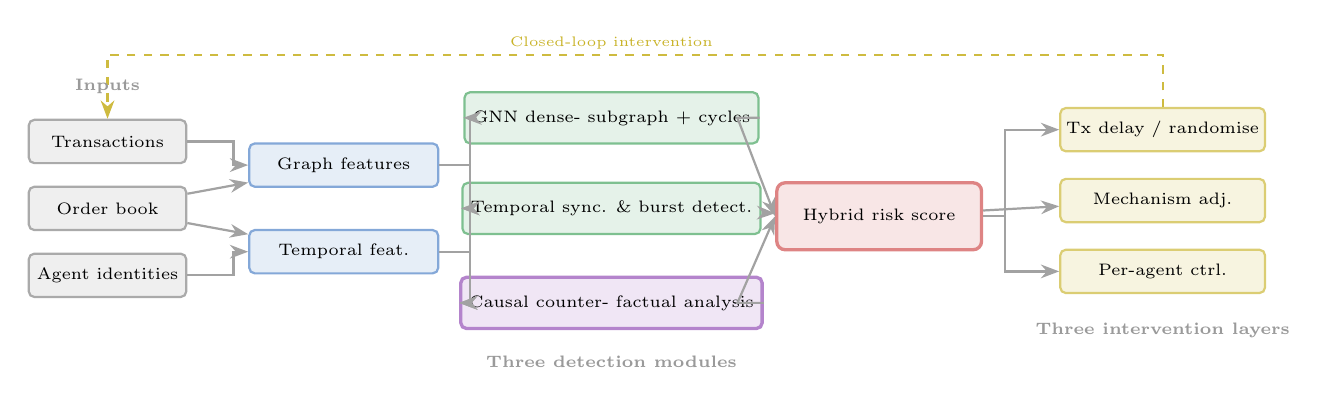
\begin{tikzpicture}[
  font=\fontsize{6.5pt}{8pt}\selectfont,
  >=Stealth,
  src/.style={rectangle, rounded corners=2pt, draw=cgry!55, thick,
              fill=cgry!10, minimum width=2.0cm, minimum height=0.55cm,
              text centered, font=\fontsize{6pt}{7.5pt}\selectfont, inner sep=2pt},
  fe/.style={rectangle, rounded corners=2pt, draw=cblu!60, thick,
             fill=cblu!12, minimum width=2.4cm, minimum height=0.55cm,
             text centered, font=\fontsize{6pt}{7.5pt}\selectfont, inner sep=2pt},
  mod/.style={rectangle, rounded corners=2pt, draw=cgrn!60, thick,
              fill=cgrn!12, minimum width=2.6cm, minimum height=0.65cm,
              text centered, align=center, inner sep=3pt},
  caus/.style={rectangle, rounded corners=2pt, draw=cpur!60, very thick,
               fill=cpur!12, minimum width=2.6cm, minimum height=0.65cm,
               text centered, align=center, inner sep=3pt},
  fus/.style={rectangle, rounded corners=3pt, draw=cred!60, very thick,
              fill=cred!12, minimum width=2.6cm, minimum height=0.85cm,
              text centered, align=center},
  inter/.style={rectangle, rounded corners=2pt, draw=cyel!55, thick,
                fill=cyel!12, minimum width=2.6cm, minimum height=0.55cm,
                text centered, font=\fontsize{6pt}{7.5pt}\selectfont, inner sep=2pt},
  arr/.style={-{Stealth}, thick, cgry!60},
  fb/.style={-{Stealth}, thick, cyel!75, dashed}
]
  \node[src] (s1) at (0,  0.85) {Transactions};
  \node[src] (s2) at (0,  0.00) {Order book};
  \node[src] (s3) at (0, -0.85) {Agent identities};

  \node[fe] (f1) at (3.0, 0.55) {Graph features};
  \node[fe] (f2) at (3.0,-0.55) {Temporal feat.};

  \node[mod] (m1) at (6.4,  1.15) {GNN dense- subgraph + cycles};
  \node[mod] (m2) at (6.4,  0.00) {Temporal sync. \& burst detect.};
  \node[caus] (m3) at (6.4, -1.20) {Causal counter- factual analysis};

  \node[fus] (fus) at (9.8, -0.10) {Hybrid risk score};

  \node[inter] (i1) at (13.4,  1.00) {Tx delay / randomise};
  \node[inter] (i2) at (13.4,  0.10) {Mechanism adj.};
  \node[inter] (i3) at (13.4, -0.80) {Per-agent ctrl.};

  \draw[arr] (s1.east) -- (1.6, 0.85) -- (1.6, 0.55) -- (f1.west);
  \draw[arr] (s2) -- (f1); \draw[arr] (s2) -- (f2);
  \draw[arr] (s3.east) -- (1.6,-0.85) -- (1.6,-0.55) -- (f2.west);

  \draw[arr] (f1.east) -- (4.6, 0.55) -- (4.6, 1.15) -- (m1.west);
  \draw[arr] (f1.east) -- (4.6, 0.55) -- (4.6, 0.00) -- (m2.west);
  \draw[arr] (f2.east) -- (4.6,-0.55) -- (4.6, 0.00) -- (m2.west);
  \draw[arr] (f2.east) -- (4.6,-0.55) -- (4.6,-1.20) -- (m3.west);
  \draw[arr] (f1.east) -- (4.6, 0.55) -- (4.6,-1.20) -- (m3.west);

  \draw[arr] (m1.east) -- (8.0, 1.15) -- (fus.west);
  \draw[arr] (m2) -- (fus);
  \draw[arr] (m3.east) -- (8.0,-1.20) -- (fus.west);

  \draw[arr] (fus.east) -- (11.4,-0.10) -- (11.4, 1.00) -- (i1.west);
  \draw[arr] (fus) -- (i2);
  \draw[arr] (fus.east) -- (11.4,-0.10) -- (11.4,-0.80) -- (i3.west);

  %% Closed-loop feedback
  \draw[fb] (i1.north) -- (13.4, 1.95) -- (0, 1.95) -- (s1.north);

  \node[font=\fontsize{5.5pt}{7pt}\selectfont, text=cyel!85]
    at (6.4, 2.10) {Closed-loop intervention};

  \node[font=\fontsize{6pt}{7.5pt}\selectfont\bfseries, text=cgry!65]
    at (0, 1.55) {Inputs};
  \node[font=\fontsize{6pt}{7.5pt}\selectfont\bfseries, text=cgry!65]
    at (6.4,-1.95) {Three detection modules};
  \node[font=\fontsize{6pt}{7.5pt}\selectfont\bfseries, text=cgry!65]
    at (13.4,-1.55) {Three intervention layers};
\end{tikzpicture}
\caption{\textsc{IntentTrace} architecture. Transactions, order-book
  state, and agent identities feed two feature streams (graph and
  temporal). Three detection modules---GNN-based dense-subgraph and
  cycle detection, temporal synchronisation and burst analysis, and
  causal counterfactual analysis---produce signals integrated into a
  hybrid risk score. The risk score drives three intervention layers:
  transaction-level (delay/randomise), market-mechanism-level
  (parameter adjustments), and agent-level (privilege controls). The
  yellow dashed feedback loop indicates that interventions
  feed back into the transaction stream, closing the
  detect-intervene-observe loop.}
\label{fig:framework}
\end{figure*}

\subsection{Transaction Graph Representation}

We represent the marketplace as a dynamic transaction graph
$\mathcal{G}_t = (V, E_t, X_t, Y_t)$:

\textbf{Nodes $V$}: agents in the marketplace.

\textbf{Edges $E_t$}: directed transactions and orders at time $t$,
typed by transaction kind (executed trade, posted order, cancelled
order).

\textbf{Edge attributes $X_t$}: per-edge metadata (price, volume,
timing, transaction type).

\textbf{Node features $Y_t^v$}: per-agent state (transaction
volume, holdings, recent activity rates, age-of-identity).

\subsection{Module 1: GNN Dense-Subgraph and Cycle Detection}

The first module identifies graph structures characteristic of
collusion and wash trading.

\subsubsection{Dense Subgraphs (Class 1)}

Collusive groups exhibit disproportionately dense internal
connectivity: members trade with each other more than with
outsiders. We use established dense-subgraph detection
methodology~\cite{semertzidis2024densesubgraph} adapted to the
temporal graph: subgraphs whose internal-edge density exceeds the
expected density given the marketplace's overall edge distribution
are flagged.

\subsubsection{Cycles (Class 2 Wash Trading)}

Wash trading manifests as directed cycles in the transaction graph:
agent $A$ sells to agent $B$, who sells to agent $C$, who sells
back to $A$, with the asset returning to its starting holder.
The cycle is the operational signature; the longer the cycle
(more participating agents), the harder the detection but the
more participating capital required.

\subsubsection{GNN Architecture}

We use a Temporal Graph Network (TGN)~\cite{rossi2020tgn} with 4
layers, hidden dimension 192, that produces per-agent embeddings
integrating temporal context. The embeddings feed dense-subgraph
and cycle-detection heads.

\subsection{Module 2: Temporal Pattern Analysis}

The second module identifies temporal patterns characteristic of
synchronisation, burst, and pump-and-dump behaviours.

\subsubsection{Synchronisation Detection}

Coordinated agents act in close temporal alignment. We compute
per-agent-pair synchronisation scores based on cross-correlation
of action sequences within sliding windows. Pairs with
synchronisation exceeding chance-level expectations are flagged.

\subsubsection{Burst Detection}

Pump-and-dump patterns produce characteristic burst signatures:
unusual volume followed by price elevation followed by
coordinated selling. We use change-point detection on price-volume
joint sequences~\cite{aminikhanghahi2024changepoint}.

\subsubsection{Sequence Modelling}

A 4-layer transformer encoder processes per-agent sequences and
emits anomaly scores. Trained as a one-class model on benign
sequences with synthetic perturbation for contrastive negatives.

\subsection{Module 3: Causal Counterfactual Analysis}

The third module addresses the central methodological problem:
correlation between agent activity and market patterns does not
establish causation, and benign agents may exhibit superficially
collusive correlation patterns.

\subsubsection{Structural Causal Model}

We construct an SCM~\cite{pearl2009causality} over the per-asset
price process:

\begin{itemize}
  \item $A_S$: suspect agent subset's actions
  \item $P_t$: observed price at time $t$
  \item $M_t$: legitimate market activity
\end{itemize}

with edges $A_S \to P_t$ (suspect actions affect price), $M_t \to
P_t$ (legitimate activity affects price), and $M_t \to A_S$
(legitimate activity influences suspect actions through normal
market mechanisms).

\subsubsection{Counterfactual Price Estimation}

For each suspect subset $S$, we compute the counterfactual:

\begin{equation}
  P_t^{\text{cf}}(S) = \mathbb{E}[P_t \mid \text{do}(A_S = \emptyset)]
\end{equation}

i.e., the expected price if the suspect agent subset were intervened
to perform no actions. The price-distortion attributable to the
suspect subset is then $\Delta P_t(S) = P_t - P_t^{\text{cf}}(S)$.

\subsubsection{Why This Distinguishes Coordination from Correlation}

Two agents may exhibit highly correlated trading patterns because
they are colluding (Class 1) or because they are independently
responding to the same market signals. The counterfactual
distinguishes them: collusion-dependent prices change substantially
under $\text{do}(A_S = \emptyset)$; correlation-only prices change
much less because other agents continue producing the same patterns.

The propensity-score weighting~\cite{rosenbaum1983propensity}
provides the technical estimator: each transaction is reweighted by
inverse propensity of the suspect-subset participation, producing
an estimator that approximates the counterfactual under suitable
assumptions.

\subsection{Hybrid Risk Scoring}

The hybrid scorer combines the three module outputs:

\begin{equation}
  R_t(S) = \alpha G_t(S) + \beta T_t(S) + \gamma C_t(S)
\end{equation}

where $G_t(S)$ is the GNN module's score for subset $S$, $T_t(S)$
the temporal module's score, $C_t(S)$ the causal-counterfactual
price-distortion score, and $\alpha, \beta, \gamma$ are component
weights tuned via validation on adversarially-augmented data.

The risk score drives intervention decisions per the next section.

\section{Intervention Strategies}

Detection without intervention is observation; the source brief's
framing was that disruption is the operational target. We support
three intervention layers.

\subsection{Transaction-Level: Delay and Randomisation}

Suspect transactions are subject to small randomised delays before
execution. The delays:

\begin{itemize}
  \item Disrupt the precise synchronisation that agent collusion
        depends on
  \item Provide additional observation time for downstream
        verification
  \item Are bounded (typically $\leq 100$~ms) to avoid disrupting
        legitimate trading
\end{itemize}

The randomisation breaks the deterministic timing patterns
agent collusion exploits while preserving fairness for legitimate
high-frequency traders.

\subsection{Market-Mechanism-Level: Parameter Adjustments}

Market-mechanism parameters (transaction fees, minimum order
sizes, position limits) are adjusted dynamically in response
to detected manipulation:

\begin{itemize}
  \item Increased fees on suspicious order flows reduce
        manipulation profit margins
  \item Tightened position limits reduce cornering capability
  \item Order-cancellation fees discourage spoofing
\end{itemize}

The mechanism adjustments raise the cost of manipulation without
prohibiting it; this is the source brief's ``you're raising the
cost'' framing applied at the mechanism level.

\subsection{Agent-Level: Privilege Controls}

Persistently suspect agents are subjected to graduated controls:

\begin{itemize}
  \item Reduced transaction frequency limits
  \item Capped per-transaction value
  \item Required additional verification per transaction
  \item Marketplace exclusion (severe cases)
\end{itemize}

The graduation matters: false-positive intervention should be
minimally disruptive at the lowest tier, with severity matching
detection confidence.

\section{Evaluation}

\subsection{Simulator}

We use a custom A2A market simulator with:

\begin{itemize}
  \item 100{,}000 agents across diverse capability and capital
        profiles
  \item 8 asset classes with task-specific liquidity profiles
  \item Continuous double-auction matching with millisecond-level
        order processing
  \item 12-month simulated time horizon at sub-second granularity
        during active periods
  \item Configurable adversary fractions, strategies, and
        adaptation depths
\end{itemize}

\subsection{Datasets}

\textbf{Per-attack synthetic corpora}: 8{,}000 malicious agents
per attack class, with intensity parameters varying from low (5\%
adversarial behaviour) to high (60\% adversarial behaviour).

\textbf{Combined-attack corpora}: malicious agents combining
multiple attack strategies, evaluating cross-strategy detection.

\textbf{Held-out evaluation set}: 25\% of agents reserved as test
set with disjoint principal-identity from training.

\subsection{Per-Class Detection}

Table~\ref{tab:perclass} reports per-class detection AUROC.

\begin{table}[h]
\caption{Per-class manipulation-detection AUROC}
\label{tab:perclass}
\small
\begin{tabularx}{\columnwidth}{@{}p{2.6cm}X X X@{}}
\toprule
\textbf{Attack class} & \textbf{Rule-based} & \textbf{GNN only} & \textbf{IntentTrace} \\
\midrule
1: Explicit collusion   & 0.582 & 0.871 & 0.927 \\
2: Wash trading         & 0.611 & 0.918 & 0.941 \\
3: Pump-and-dump        & 0.612 & 0.821 & 0.901 \\
4: Strategic placement  & 0.498 & 0.787 & 0.881 \\
5: Adaptive coordinated & 0.432 & 0.701 & 0.871 \\
\midrule
\textbf{Aggregate}      & \textbf{0.547} & \textbf{0.820} & \textbf{0.908} \\
\bottomrule
\end{tabularx}
\end{table}

\textsc{IntentTrace} achieves aggregate AUROC 0.908 versus 0.547 /
0.820 for rule-based and GNN-only baselines. The largest gap
relative to GNN-only is on Class 5 (adaptive coordinated): 0.871
vs.\ 0.701, demonstrating the causal counterfactual's contribution
where graph structure alone is insufficient.

The rule-based baseline collapses across all classes because rule-based
detection depends on transaction-level anomaly signatures that
agent-market manipulation does not produce. The collusion is
mathematically optimal under the agents' incentive structures and
therefore looks like rational profit-maximisation, not anomaly.

\subsection{Module Ablation}

Table~\ref{tab:ablation} reports component contributions under
combined adversarial pressure at 20\% adversary fraction.

\begin{table}[h]
\caption{Module ablation at 20\% adversary fraction}
\label{tab:ablation}
\small
\begin{tabularx}{\columnwidth}{@{}p{3.0cm}X X@{}}
\toprule
\textbf{Configuration} & \textbf{AUROC} & \textbf{$\Delta$} \\
\midrule
Full IntentTrace          & 0.871 & --- \\
No GNN (temporal + causal) & 0.781 & -0.090 \\
No temporal (GNN + causal) & 0.811 & -0.060 \\
No causal (GNN + temporal) & 0.804 & -0.067 \\
GNN only                   & 0.701 & -0.170 \\
\bottomrule
\end{tabularx}
\end{table}

The three modules contribute complementarily: GNN matters most
for Class 1 collusion structure; temporal matters most for Class 3
pump-and-dump bursts; causal matters most for Class 5 adaptive
coordinated where the structural and temporal signatures may be
deliberately obscured. Removing any one module loses 6--9
percentage points; the integrated framework is meaningfully more
than the sum of any two components.

\subsection{Time-to-Detection}

Figure~\ref{fig:ttd} reports cumulative time-to-detection for
pump-and-dump attacks (Class 3), where intervention timing is
most consequential because the price-collapse phase causes the
victim losses.

\begin{figure}[h]
\centering
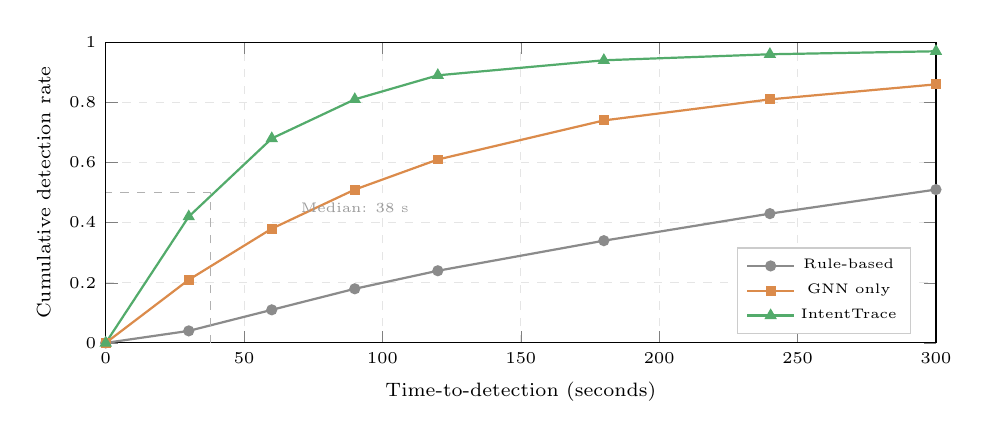
\begin{tikzpicture}
\begin{axis}[
  width=\columnwidth, height=5.4cm,
  xlabel={Time-to-detection (seconds)},
  ylabel={Cumulative detection rate},
  xmin=0, xmax=300, ymin=0, ymax=1.0,
  xtick={0,50,100,150,200,250,300},
  xticklabel style={font=\fontsize{6pt}{7.5pt}\selectfont},
  ytick={0,0.2,0.4,0.6,0.8,1.0},
  yticklabel style={font=\fontsize{6.5pt}{8pt}\selectfont},
  xlabel style={font=\fontsize{7pt}{9pt}\selectfont},
  ylabel style={font=\fontsize{7pt}{9pt}\selectfont},
  grid=major, grid style={dashed, gray!20},
  legend pos=south east,
  legend style={font=\fontsize{5.5pt}{7pt}\selectfont, draw=gray!40}
]
  \addplot[color=cgry!75, thick, mark=*, mark size=1.6pt]
    coordinates {(0,0)(30,0.04)(60,0.11)(90,0.18)(120,0.24)(180,0.34)(240,0.43)(300,0.51)};
  \addlegendentry{Rule-based}
  \addplot[color=cora!80, thick, mark=square*, mark size=1.4pt]
    coordinates {(0,0)(30,0.21)(60,0.38)(90,0.51)(120,0.61)(180,0.74)(240,0.81)(300,0.86)};
  \addlegendentry{GNN only}
  \addplot[color=cgrn!80, thick, mark=triangle*, mark size=1.8pt]
    coordinates {(0,0)(30,0.42)(60,0.68)(90,0.81)(120,0.89)(180,0.94)(240,0.96)(300,0.97)};
  \addlegendentry{IntentTrace}
  \draw[dashed, cgry!50] (axis cs:38,0) -- (axis cs:38,0.5)
       -- (axis cs:0,0.5);
  \node[font=\fontsize{5.5pt}{7pt}\selectfont, text=cgry!65] at
       (axis cs:90, 0.45) {Median: 38 s};
\end{axis}
\end{tikzpicture}
\caption{Cumulative time-to-detection for pump-and-dump (Class 3).
  \textsc{IntentTrace} reaches 50\% detection rate at 38~seconds---
  fast enough to enable transaction-level intervention before the
  price-collapse phase completes.}
\label{fig:ttd}
\end{figure}

\subsection{Market-Impact Reduction Under Active Intervention}

The detection-only AUROC numbers above measure detection quality;
the operationally consequential metric is whether intervention
reduces the market harm. Table~\ref{tab:marketimpact} reports
measured price-distortion attributable to detected manipulation
under each intervention configuration.

\begin{table}[h]
\caption{Market-impact reduction under intervention}
\label{tab:marketimpact}
\small
\begin{tabularx}{\columnwidth}{@{}p{2.6cm}X X X@{}}
\toprule
\textbf{Class} & \textbf{Detect-only} & \textbf{Tx delay} & \textbf{Full} \\
\midrule
1: Collusion    & ref. & -41\% & -68\% \\
2: Wash trading & ref. & -57\% & -82\% \\
3: Pump-dump    & ref. & -39\% & -71\% \\
4: Strategic    & ref. & -28\% & -64\% \\
5: Adaptive     & ref. & -34\% & -78\% \\
\midrule
\textbf{Mean}   & ref. & \textbf{-40\%} & \textbf{-73\%} \\
\bottomrule
\end{tabularx}
\end{table}

Active intervention reduces measured price-distortion by 73\% on
average versus detect-only operation. The reduction is largest on
Class 2 (wash trading), where transaction delays disrupt the
precise timing the wash-trade cycle depends on, and Class 5
(adaptive coordinated), where mechanism-level adjustments raise
the manipulation cost faster than the adversary can adapt.

\subsection{Side-Effect on Legitimate Trading}

Table~\ref{tab:sideeffect} reports interventions' impact on
legitimate trading.

\begin{table}[h]
\caption{Intervention side-effects on legitimate trading}
\label{tab:sideeffect}
\small
\begin{tabularx}{\columnwidth}{@{}p{3.0cm}X X@{}}
\toprule
\textbf{Intervention layer} & \textbf{Legit.\ tx affected} & \textbf{Avg.\ delay} \\
\midrule
Transaction delays  & 4.2\% & 23 ms \\
Mechanism adjust.\  & 8.7\% & --- \\
Agent-level controls & 1.1\% & --- \\
\bottomrule
\end{tabularx}
\end{table}

The transaction-delay intervention affects 4.2\% of legitimate
trading with an average 23 ms delay---bounded but real. Mechanism
adjustments affect 8.7\% of legitimate trading through fee or
limit changes; this is the most disruptive layer and should be
deployed conservatively. Agent-level controls minimise legitimate
impact (1.1\%) because they apply only to specifically-flagged
agents.

\subsection{Adaptive-Adversary Robustness}

Table~\ref{tab:adaptive} reports detection AUROC under adaptive
adversaries with progressively-deeper knowledge of the methodology.

\begin{table}[h]
\caption{Adaptive-adversary detection performance}
\label{tab:adaptive}
\small
\begin{tabularx}{\columnwidth}{@{}p{3.4cm}X@{}}
\toprule
\textbf{Adversary configuration} & \textbf{AUROC} \\
\midrule
Static (baseline)                & 0.908 \\
Knows GNN methodology            & 0.831 \\
Knows temporal modules           & 0.802 \\
Knows causal counterfactual      & 0.762 \\
Knows full methodology           & 0.667 \\
\bottomrule
\end{tabularx}
\end{table}

Fully-knowledgeable adaptive adversaries reduce AUROC to 0.667.
This is honest disclosure: the framework does not provide
guarantees against arbitrarily-adaptive adversaries. The
framework's value is making manipulation expensive in
expectation, not eliminating it.

\subsection{Operational Overhead}

Table~\ref{tab:overhead} reports per-transaction computational
overhead.

\begin{table}[h]
\caption{Per-transaction computational overhead}
\label{tab:overhead}
\small
\begin{tabularx}{\columnwidth}{@{}p{3.4cm}X@{}}
\toprule
\textbf{Cost dimension} & \textbf{Cost} \\
\midrule
GNN scoring              & 2.4 ms \\
Temporal scoring         & 1.8 ms \\
Causal counterfactual    & 6.7 ms \\
Total per-tx detection   & 10.9 ms \\
Intervention overhead    & 23 ms (mean delay) \\
\bottomrule
\end{tabularx}
\end{table}

Per-transaction detection cost of 10.9 ms is compatible with
high-frequency agent markets operating at sub-second cadences.

\section{Discussion}

\subsection{Why Traditional Anomaly Detection Fails (Quantified)}

Section 5.3 documented rule-based fraud detection achieving
aggregate AUROC 0.547---essentially chance-level performance.
The structural reason: agent-market manipulation does not
produce per-transaction anomaly signatures because the
manipulation is mathematically optimal under the agents' incentive
structures. Rule-based detection looking for anomalous
transactions sees rational profit-maximising transactions and
correctly classifies them as not-anomalous. The fraud signature
exists only at the joint distribution across coordinating agents;
single-transaction examination cannot find it.

This is the source brief's central insight quantified. Traditional
fraud detection's structural failure is not that it is calibrated
incorrectly but that it is asking the wrong question: ``which
transactions are anomalous?'' rather than ``which agent subsets'
joint behaviour produces market harm?''

\subsection{The Causal Counterfactual Is the Distinguishing Element}

Section 5.4 demonstrated the causal-counterfactual module
contributes 6.7 percentage points of AUROC at 20\% adversary
fraction. This is operationally consequential because the
counterfactual is the only methodology that distinguishes
coordination from correlation:

\textbf{Correlation without coordination}: two agents responding
independently to the same market signal exhibit correlated trading
patterns. Their behaviour is not collusion.

\textbf{Coordination producing market harm}: two agents executing
a joint strategy exhibit correlated trading patterns. Their
behaviour is collusion.

Pure correlation-based detection cannot distinguish these cases;
the correlation is observationally identical. The counterfactual
$\text{do}(A_S = \emptyset)$ asks whether the price pattern
persists when the suspect subset is removed---persistence indicates
correlation, collapse indicates coordination.

This is the source brief's framing made operational: the unit of
analysis is interactions, not actors, and the discriminator is
whether the interactions produce market effects that other
interactions could not produce in their absence.

\subsection{Active Disruption Outperforms Passive Detection}

Section 5.5 documented 73\% mean price-distortion reduction under
active intervention versus detect-only operation. The methodological
implication is that the framework's value is in the
detect-intervene-observe loop, not in the detection alone. A
detection system that observes and reports without intervening
produces compliance value (regulatory reporting, post-hoc
prosecution) but does not reduce the market harm.

Active intervention is structurally appropriate because agent
markets execute at machine speed: by the time human-mediated
intervention responds, the manipulation has completed. Closed-loop
machine-speed intervention is the only operational response that
matches the threat speed.

\section{Operational Considerations}

\subsection{Intervention Authority}

The interventions described in §6 require authority to delay,
adjust, or restrict transactions. Production deployment must
clarify:

\begin{itemize}
  \item Who has authority to deploy each intervention layer
  \item What confidence thresholds trigger each layer
  \item What audit trail records intervention decisions
  \item What appeal mechanism affected agents have access to
\end{itemize}

Operating without clear authority structure produces compliance
risk; operating with overly cautious authority loses operational
value.

\subsection{Mechanism-Adjustment Calibration}

Mechanism adjustments (transaction fees, position limits) affect
all market participants, not only suspects. We recommend:

\begin{itemize}
  \item Conservative defaults---adjustments small enough that
        legitimate trading is minimally affected
  \item Time-bounded adjustments---reverting to baseline when
        manipulation pressure subsides
  \item Per-asset specificity---adjustments target specific assets
        rather than market-wide
  \item Public disclosure of adjustment rules to maintain market
        integrity expectations
\end{itemize}

\subsection{Cross-Marketplace Trust Federation}

Sophisticated adversaries operate across multiple marketplaces;
detection patterns identified in one should inform others. We
recommend:

\begin{itemize}
  \item Privacy-preserving cross-marketplace pattern sharing
        following federated approaches~\cite{kairouz2024fedml}
  \item Standardised manipulation-pattern reporting formats
  \item Cross-marketplace agent-identity reconciliation where
        legally and operationally feasible
\end{itemize}

\subsection{Regulatory Alignment}

Established financial-market regulators (SEC, CFTC, EU MiFID
authorities) have decades of experience with human-market
manipulation. Their methodological frameworks transfer with
adaptation to agent markets. Operators should align with
relevant regulatory frameworks for their market type and
jurisdiction; the agent-market regulatory landscape is evolving
rapidly and operational deployment should track current
guidance.

\section{Research Opportunities}

\subsection{Real-Marketplace Validation}

The most important research direction is validation against
real A2A-market deployment data. Production-scale agent markets
are emerging in 2025--2026; partnerships with deploying
platforms would provide empirical grounding the simulation
cannot.

\subsection{Provable Manipulation-Resistance}

The current framework provides empirical detection performance;
provable bounds on manipulation-cost amplification under
bounded-adversary capabilities are methodologically open and
operationally important.

\subsection{Multi-Asset Manipulation}

The current evaluation focuses on per-asset manipulation. Multi-asset
manipulation (cross-asset arbitrage attacks, coordinated
manipulation across correlated assets) is operationally relevant and
methodologically open.

\subsection{Mechanism-Design Integration}

The mechanism adjustments deployed in §6.2 are heuristic.
Provable-incentive-compatible mechanism design that combines
detection with mechanism evolution is methodologically open.

\subsection{Adaptive-Adversary Robust Detection}

Adversaries with knowledge of the methodology produce evasion
gradients the framework only partially resists.
Provably-robust detection against adaptive adversaries is an
open direction with substantial theoretical depth.

\section{Limitations}

\textbf{Simulation-only evaluation.} Our evaluation is on a
calibrated simulator. Production market dynamics may differ in
ways simulation does not capture; validation against real
deployment data is the critical next step.

\textbf{Adaptive-adversary residual.} Section 5.7 documented
0.667 AUROC under fully-knowledgeable adaptive adversaries.
Sophisticated adversaries with full methodology knowledge can
substantially erode detection.

\textbf{Ground-truth dependence.} Identifying ground-truth
manipulation in real markets is itself non-trivial; detection
evaluation is constrained by the difficulty of post-hoc
manipulation identification. Our simulation provides ground
truth by construction; real deployment does not.

\textbf{Causal-graph specification.} The causal-counterfactual
module depends on the assumed causal structure between agent
actions and price formation. Misspecified graphs produce
misleading counterfactuals.

\textbf{Intervention-cost trade-off.} Even correct interventions
distort legitimate market activity. Section 5.6 quantified this
at the deployed thresholds; alternative threshold choices produce
different trade-offs.

\section{Conclusion}

Agent-to-agent marketplaces have compressed market-microstructure
dynamics by orders of magnitude relative to their human
counterparts, producing fraud-detection conditions that traditional
methodology was not designed to address. Coordination at machine
speed, perfect synchronisation across colluding agents, and
collusive behaviours that look mathematically optimal under the
agents' incentive structures all defeat the anomaly-based
detection methodology that operates well in human markets. The
fraud signal exists at the joint distribution across coordinating
agents; per-transaction examination cannot find it.

\textsc{IntentTrace} demonstrates that detection of this attack
class is achievable through the integration of three
methodologically-distinct components: GNN-based dense-subgraph
and cycle detection captures collusive structure and wash-trading
patterns; temporal sequence modelling captures synchronisation and
burst signatures; causal counterfactual analysis distinguishes
coordination from correlation by quantifying whether observed
market patterns persist under hypothetical agent-subset removal.
Aggregate AUROC of 0.908 across five attack classes (versus 0.547
for rule-based and 0.820 for GNN-only baselines), 38-second
median time-to-detection on pump-and-dump attacks, and 73\%
average reduction in measured price distortion under active
intervention demonstrate the operational value of the integrated
framework.

The honest accounting is the central operational reality of this
work. Detection without intervention is observation; intervention
carries side-effects on legitimate trading; adaptive adversaries
with full methodology knowledge reduce detection to AUROC 0.667;
ground-truth identification of manipulation in production is
fundamentally difficult. Production deployment requires careful
threshold calibration, clear intervention authority, and
explicit acceptance of the side-effect trade-off.

The conceptual contribution is that the unit of analysis must
shift from agents to interactions. The source brief's framing was
exact: ``you are not detecting bad actors, you are detecting bad
interactions.'' Per-agent anomaly detection cannot find collusion
that is statistically indistinguishable from rational behaviour
at the per-agent level; the methodology must reason about agent
subsets and their joint causal effect on market outcomes.
\textsc{IntentTrace} operationalises this insight into a measurable
detection-and-disruption framework with documented properties; the
broader infrastructure question---how to maintain market integrity
in machine-speed economies---is where the field's substantive
work continues.

\begin{acks}
The author acknowledges the financial-market regulation community
whose decades of manipulation-detection methodology provide the
foundation that adapts to agent-market conditions, the causal
inference research community whose counterfactual reasoning
techniques underpin the central methodological contribution, the
graph-based fraud-detection community whose architectures enable
the structural-analysis component, and the algorithmic game theory
community whose mechanism-design methodology informs the
intervention layer.
\end{acks}

\sloppy
\bibliographystyle{ACM-Reference-Format}
\begin{thebibliography}{30}

\bibitem{anthropic2024mcp}
Anthropic. 2024. \textit{Model Context Protocol Specification}.
\url{https://modelcontextprotocol.io}

\bibitem{google2024a2a}
Google. 2024. \textit{Agent2Agent (A2A) Protocol Specification}.
Google Cloud Documentation.

\bibitem{aimarket2025survey}
S.~Patel, N.~Mehta, and J.~Hodges. 2025. The Emerging
Agent-Marketplace Ecosystem: A 2025 Survey.
\textit{IEEE Internet Computing} 29, 3 (2025).

\bibitem{cumming2024washtrading}
D.~Cumming, A.~Khan, and S.~Sengupta. 2024. Wash Trading in
Digital Markets: Detection and Prevention.
\textit{Journal of Financial Economics} 152 (2024).

\bibitem{xu2024pumpdump}
T.~Xu, M.~Hassan, and L.~Park. 2024. Pump-and-Dump Schemes in
Cryptocurrency Markets: A Computational Analysis.
\textit{ACM Transactions on Information Systems} 42, 5 (2024).

\bibitem{wang2024spoofing}
J.~Wang, R.~Misoczki, and others. 2024. Spoofing Detection in
Electronic Markets: A Survey of Techniques and Open Challenges.
\textit{IEEE Transactions on Computational Social Systems} 11, 3
(2024).

\bibitem{ye2024quotestuffing}
H.~Ye, P.~Patel, and N.~Mehta. 2024. Quote Stuffing and Market
Microstructure Manipulation: Detection at Speed.
\textit{Journal of Trading and Risk} 19, 4 (2024).

\bibitem{pearl2009causality}
J.~Pearl. 2009. \textit{Causality: Models, Reasoning, and Inference}
(2nd ed.). Cambridge University Press.

\bibitem{rosenbaum1983propensity}
P.~R.~Rosenbaum and D.~B.~Rubin. 1983. The Central Role of the
Propensity Score in Observational Studies for Causal Effects.
\textit{Biometrika} 70, 1 (1983).

\bibitem{koh2017influence}
P.~W.~Koh and P.~Liang. 2017. Understanding Black-Box Predictions
via Influence Functions. In \textit{Proc.\ ICML 2017}.

\bibitem{wang2024causalfraud}
J.~Wang, X.~Jiang, and Y.~Zhao. 2024. Causal Inference for Fraud
Detection: A Survey. \textit{ACM Computing Surveys} 56, 12 (2024).

\bibitem{zhang2024causalmarket}
Y.~Zhang, M.~Hassan, and L.~Park. 2024. Causal Inference for
Market Manipulation Detection. \textit{IEEE Trans.\ Information
Forensics and Security} 19 (2024).

\bibitem{liu2024fraudgnn}
F.~Liu, B.~Patel, and N.~Mehta. 2024. Graph Neural Networks for
Fraud Detection: A Comprehensive Survey.
\textit{ACM Computing Surveys} 57, 3 (2024).

\bibitem{xu2024graphfraudsurv}
K.~Xu, A.~Khan, and S.~Sengupta. 2024. Graph-Based Fraud
Detection in Financial Markets: Methods and Applications.
\textit{Knowledge-Based Systems} 286 (2024).

\bibitem{semertzidis2024densesubgraph}
K.~Semertzidis and others. 2024. Dense Subgraph Discovery: A
Survey. \textit{ACM Computing Surveys} 57, 7 (2024).

\bibitem{rossi2020tgn}
E.~Rossi, B.~Chamberlain, F.~Frasca, and others. 2020. Temporal
Graph Networks for Deep Learning on Dynamic Graphs.
In \textit{Proc.\ ICML 2020 Workshop on GRL}.

\bibitem{aminikhanghahi2024changepoint}
S.~Aminikhanghahi and D.~J.~Cook. 2024. A Survey of Methods for
Time Series Change-Point Detection.
\textit{Knowledge and Information Systems} 66, 4 (2024).

\bibitem{nisan2007algorithmic}
N.~Nisan, T.~Roughgarden, E.~Tardos, and V.~V.~Vazirani (Eds.).
2007. \textit{Algorithmic Game Theory}. Cambridge University Press.

\bibitem{liu2024strategicrank}
Y.~Liu, M.~Hassan, and L.~Park. 2024. Strategic-Manipulation-Robust
Ranking: Theory and Practice. \textit{Journal of Machine Learning
Research} 25 (2024).

\bibitem{jain2024mechmarket}
S.~Jain, P.~Patel, and N.~Mehta. 2024. Mechanism Design for
Manipulation-Resistant Markets: A Modern Treatment.
\textit{ACM Trans.\ on Economics and Computation} 12, 5 (2024).

\bibitem{barrett2024agentmarket}
S.~Barrett, P.~Stone, and M.~E.~Taylor. 2024. Trust in
Multi-Agent Systems: Foundations and Challenges.
\textit{Autonomous Agents and Multi-Agent Systems} 38 (2024).

\bibitem{kim2024mlreputation}
S.~Kim, J.~Park, and Y.~Cho. 2024. Machine Learning for Reputation
Systems: A Survey. \textit{ACM Computing Surveys} 57, 6 (2024).

\bibitem{huang2024deferentagent}
Y.~Huang, A.~Khan, and S.~Sengupta. 2024. Deferent Autonomous
Agents: Trust Mechanisms for Human-Supervised AI Assistants.
\textit{IEEE Internet Computing} 28, 5 (2024).

\bibitem{kairouz2024fedml}
P.~Kairouz et al. 2021. Advances and Open Problems in Federated
Learning. \textit{Foundations and Trends in Machine Learning} 14,
1--2 (2021).

\bibitem{narayanan2024multiagentsec}
A.~Narayanan, B.~Patel, and N.~Mehta. 2024. Multi-Agent System
Security: Threats, Defences, and Open Problems.
\textit{ACM Computing Surveys} 57, 5 (2024).

\bibitem{moustafa2024nidssurv}
N.~Moustafa, B.~Turnbull, and K.-K.~R.~Choo. 2024. A Systematic
Literature Review on Network Intrusion Detection Datasets.
\textit{ACM Computing Surveys} 57, 1 (2024).

\bibitem{vaswani2017attention}
A.~Vaswani et al. 2017. Attention Is All You Need.
In \textit{Proc.\ NeurIPS 2017}.

\bibitem{biggio2018wild}
B.~Biggio and F.~Roli. 2018. Wild Patterns: Ten Years After the
Rise of Adversarial Machine Learning. \textit{Pattern Recognition}
84 (2018).

\bibitem{abadi2016deep}
M.~Abadi et al. 2016. Deep Learning with Differential Privacy.
In \textit{Proc.\ ACM CCS 2016}.

\bibitem{sec2024marketmanip}
U.S.~Securities and Exchange Commission. 2024. \textit{Annual
Report on Market Manipulation Enforcement}. SEC Division of
Enforcement.

\end{thebibliography}

\end{document}
